\documentclass{hedexams}
\usepackage[utf8]{inputenc}
\usepackage[russian]{babel}
\usepackage[derivative]{hedmaths}
\usepackage{amsmath}
\usepackage{graphicx}
\begin{document}
    \tableofcontents
    \question{Тепловое излучение. Закон Релея-Джинса. Гипотеза Планка.
Кванты излучения. Функция Кирхгофа. Законы Стефана-Больцмана и
смещения Вина}

\subquestion{Тепловое излучение. Основные понятия}
Всё излучение делится на два типа: тепловое излучение и люминесценцию.

Тепловое излучение -- излучение за счет внутренней энергии тела, оно есть
всегда.

Люминесценция -- излучение за счет других видов энергии:
\begin{itemize}
    \item хемилюминесценция -- за счет энергии химических реакций;
    \item электролюминесценция -- за счет воздействия электрическим полем;
    \item фотолюминесценция -- за счет внешнего облучения электромагнитными
        волнами.
\end{itemize}

Основные свойства теплового излучения:
\begin{enumerate}
    \item из всех видов излучения является единственным равновесным (сколько
        энергии в виде электромагнитных волн излучается с единицы площади
        в единицу времени, столько же и поглощается). Это обусловлено тем,
        что интенсивность теплового излучения возрастает с увеличением
        температуры;
    \item немонохроматичность излучаемых электромагнитных волн;
    \item неполяризованность излучаемых электромагнитных волн.
\end{enumerate}

Количественные характеристики теплового излучения:
\begin{enumerate}
    \item энергетическая светимость \( R_T \) (интегральная испускательная
        способность) -- количество энергии излучаемое телом в виде
        электромагнитного излучения с единичной площадки за единицу времени:
        \[
            R_T = \der{W}{S\ dt};
            [R_T] = \left[ \frac{\text{Дж}}{\text{м}^2\cdot\text{с}} \right] =
            \left[ \frac{\text{Вт}}{\text{м}^2} \right].
        \]
    \item спектральная испускательная способность \( r \) -- количество энергии
        излучаемое телом в виде электромагнитного излучения с единичной
        площадки за единицу времени в узкий частотный диапазон
        \( [\omega;\ \omega + d\omega] \).
        \[
            r_\omega = \der{W}{S\ dt\ d\omega} = \der{R}{\omega};
            \quad r_\lambda = \der{R}{\lambda}.
        \]
        \[
            r_\omega\ d\omega = r_\lambda\ d\lambda,\quad r_\omega =
            r_\lambda\der{\lambda}{\omega} = \frac{2\pi c}{\omega^2}r_\lambda.
        \]
    \item поглощающая способность -- безразмерная величина, равная отношению
        поглощенной телом энергии к падающей на это тело энергии в виде
        электромагнитных волн в узком частотном интервале
        \( [\omega;\ \omega + d\omega] \).
        \[
            a_\omega = \der{W_\textit{полг}}{W_\textit{пад}} = [0, \ldots, 1].
        \]
        Если \( a = 1 \) при любой температуре, то такое тело называется
        \emph{абсолютно черным}. Если какая-либо величина описывает это тело,
        то к ней добавляется индексом символ \( ^* \): \( a^*(\omega, T) = 1 \).

    Если \( a = 0 \) при любой температуре, то такое тело называется
    \text{абсолютно белым}.

    \text{Абсолютно серыми} называются тела, которые имеют постоянный
    коэффициент поглощения во всем частотном интервале:
    \( a^\textit{сер}(\omega, T) = const < 1 \).
\end{enumerate}

\subquestion{Законы теплового излучения}

Закон Кирхгофа -- отношение испускательной к поглощательной способности не
зависит от природы тела и является функцией частоты и температуры, причем эта
функция одинакова для всех тел.

\[
    \left(\frac{r(\omega, T)}{a(\omega, T)}\right)_1 =
    \left(\frac{r(\omega, T)}{a(\omega, T)}\right)_2 =
    \ldots = r^*(\omega, T) = f(\omega, T).
\]

Из этого закона есть два следствия:
\begin{enumerate}
    \item если на какой-то частоте тело излучает больше, то на этой частоте тело
        и поглощает больше:
        \[
            r_1 > r_2;\, a_1 = a_2\frac{r_1}{r_2} > a_2.
        \]
    \item среди всех тел наибольшей испускательной способностью обладает
        абсолютно черное тело:
        \[
            r(\omega, T) = r^*(\omega, T)\cdot a(\omega, T) < r^*(\omega, T).
        \]
\end{enumerate}

Экспериментально был получен вид этой функции:
\begin{figure}[h!]
    \center
    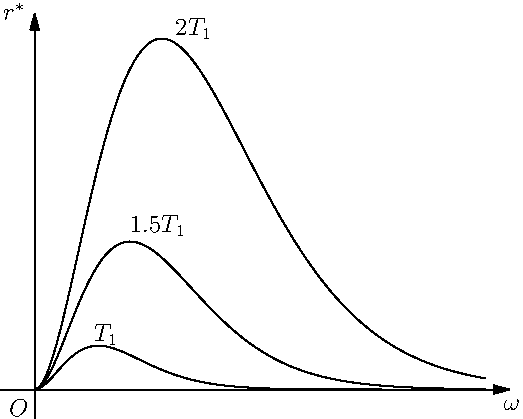
\includegraphics[width=.47\textwidth]{image}
\end{figure}

С помощью него можно установить 2 закона теплового излучения:
\begin{enumerate}
    \item закон Стефана-Больцмана -- интегральная испускательная способность
        прямо пропорциональна 4-ой степени абсолютной температуры тела;
    \item закон смещения Вина: длина волны, на которую приходится максимум
        спектральной испускательной способности абсолютно чёрного тела обратно
        пропорциональна абсолютной температуре тела.
\end{enumerate}

\subquestion{Закон Релея-Джинса}
Релеем и Джинсом была предпринята попытка определить вид функции
\( r^*(\omega, T) \). Для этого они рассмотрели кубическую полость с абсолютно
чёрными стенками. Для начала, они нашли связь между объёмной плотностью энергии
излучения и излучательной способностью фрагмента стенки:
\begin{gather*}
    dj = cu\frac{d\Omega}{4\pi},\\
    d\Phi = \vec{dj}\cdot\vec{dS} = \frac{cu}{4\pi}\cos\theta\d\Omega\,dS =
    \frac{cu}{4\pi}\cos\theta\sin\theta\d\theta\d\phi\,dS,\\
    d\Phi = \frac{cu}{4\pi}\,dS\int\limits_0^\frac{\pi}{2}\sin\theta\cos\theta
    \d\theta\int\limits_0^{2\pi}\d\phi = \frac{cu\,dS}{4},\\
    r^*(\omega, T) = \frac{d\Phi(\omega, T)}{dS} = \frac{cu(\omega, T)}{4}.
\end{gather*}
Далее они рассмотрели стенки полости как совокупность классических гармонических
осцилляторов, которые могут обмениваться энергией с излучением в полости.
Рассмотрим объёмную плотность энергии теплового излучения в полости со стороной
\( l \):
\[
    u(\omega, T) = \frac{dW}{l^3\d\omega} =
    \frac{dN\average{W(\omega, T)}}{l^3\d\omega},
\]
где \( dN \) -- число волн в спектральном диапазоне
\( [\omega, \omega+d\omega] \). Для образования стоячих волн должны выполняться
нулевые граничные условия, то есть
\[
    lk = \pi n,\ n_x = \frac{l}{\pi}k_x,\ n_y = \frac{l}{\pi}k_y,\
    n_z = \frac{l}{\pi}k_z.
\]
Число волн \( dN \), у которых \( k\in[k, k+dk] \) равно числу целых чисел в
интервале \( [n, n+dn] \):
\[
    dN = dn_x\,dn_y\,dn_z = \frac{L^3}{\pi^3}\,dk_x\,dk_y\,dk_z =
    2\frac{V}{\pi^3}\frac{4\pi k^2\,dk}{8} = \frac{V}{\pi^2}k^2\,dk =
    \frac{V}{\pi^2}\frac{\omega^2}{c^3}\,d\omega.
\]
Отсюда
\[
    u(\omega, T) =
    \frac{V}{\pi^2}\frac{\omega^2}{c^3}\frac{\average{W}}{V} =
    \frac{\omega^2}{\pi^2c^3}\average{W}.
\]
Далее Релей и Джинс предположили, что \( \average{W} = kT \) согласно
теореме о равномерном распределении энергии по степеням свободы. Таким образом,
был получен закон Релея-Джинса:
\[
    r^*(\omega, T) = \frac{\omega^2}{4\pi^2c^2}kT.
\]
Однако, полученный вид закона хорошо описывал экспериментальную зависимость лишь
при малых частотах. К тому же, он не объяснял ни закона Стефана-Больцмана, ни
закона смещения Вина.

\subquestion{Гипотеза Планка}
В 1900 году Макс Планк, понимая, что закон Релея-Джинса не содержит логических
ошибок, выдвинул гипотезу о том, что ЭМВ излучаются порциями, или квантами.
Энергия одного такого кванта зависит от частоты \( W_1 = \hbar\omega \).
Тогда осцилляторы могут иметь энергии, кратные энергии кванта:
\( W_n = n\hbar\omega \). Так как в стационарном состоянии энергия описывается
распределением Больцмана, то число осцилляторов с энергией \( W_n \) равно
\( N_n = A\cdot\exp(-W_n/kT) = A\cdot\exp(-n\hbar\omega/kT) \). Усредняя
энергию, получим
\[
    \average{W} =
    \frac{\sum\limits_{n=1}^\infty N_nW_n}{\sum\limits_{n=1}^\infty N_n} =
    \frac{\sum\limits_{n=1}^\infty A\cdot\exp(-\frac{n\hbar\omega}{kT})\cdot
    n\hbar\omega}{\sum\limits_{n=1}^\infty A\cdot\exp(-\frac{n\hbar\omega}{kT})} =
    \frac{\sum\limits_{n=1}^\infty n\exp(-\frac{n\hbar\omega}{kT})}
    {\sum\limits_{n=1}^\infty \exp(-\frac{n\hbar\omega}{kT})}\hbar\omega =
    \frac{\hbar\omega}{\exp(\frac{\hbar\omega}{kT}) - 1}.
\]
Тогда для спектральной излучательной способности абсолютно чёрного тела имеем
\[
    r^*(\omega, T) = \frac{\omega^2}{4\pi^2c^2}
    \frac{\hbar\omega}{\exp(\frac{\hbar\omega}{kT}) - 1} = \frac{\hbar\omega^3}
    {4\pi^2c^2}\frac{1}{\exp(\frac{\hbar\omega}{kT}) - 1}.
\]
Полученная Планком формула хорошо описывает экспериментальную зависимость и из
неё следуют закон Стефана-Больцмана (интегрированием) и закон смещения Вина
(дифференцированием).

\question{Оператор момента импульса}

В классической механике моментом импульса материальной точки называют векторное
произведение радиус-вектора этой точки на её импульс:
\[
    \vec{L} = \vec{r}\times\vec{p}.
\]

Аналогично можно ввести оператор момента импульса:
\[
    \hat{\vec{L}} = \hat{\vec{r}}\times\hat{\vec{p}}.
\]

Распишем этот оператор покоординатно:
\[
    \hat{\vec{L}} =
    \begin{vmatrix}
        \vec{e}_x & \vec{e}_y & \vec{e}_z \\
        x         & y         & z         \\
        \hat{p}_x & \hat{p}_y & \hat{p}_z \\
    \end{vmatrix} =
    (y\hat{p}_z - z\hat{p}_y)\vec{e}_x +
    (z\hat{p}_x - x\hat{p}_z)\vec{e}_y +
    (x\hat{p}_y - y\hat{p}_x)\vec{e}_z.
\]
Учитывая, что
\[
    \hat{p}_\alpha = -i\hbar\pder{}{\alpha}, \quad (\alpha \in \{ x,y,z \})
\]
для проекций момента импульса на декартовы оси получим:
\[
    \left\{
        \begin{array}{l}
            \hat{L}_x = -i\hbar\left( y\pder{}{z} - z\pder{}{y} \right),\\
            \hat{L}_y = -i\hbar\left( z\pder{}{x} - x\pder{}{z} \right),\\
            \hat{L}_z = -i\hbar\left( x\pder{}{y} - y\pder{}{x} \right).\\
        \end{array}
    \right.
\]
Запишем теперь коммутационные соотношения для проекций момента:
\begin{gather*}
    \left[\hat{L}_x, \hat{L}_y\right] = \hat{L}_x\hat{L}_y - \hat{L}_y\hat{L}_x=
    (y\hat{p}_z - z\hat{p}_y)(z\hat{p}_x - x\hat{p}_z) -
    (z\hat{p}_x - x\hat{p}_z)(y\hat{p}_z - z\hat{p}_y) =\\
    =(y\hat{p}_z z\hat{p}_x - xy\hat{p}_z^2 - z^2\hat{p}_y\hat{p}_x +
    z\hat{p}_y x\hat{p}_z) -
    (z\hat{p}_x y\hat{p}_z - xy\hat{p}_z^2 - z^2\hat{p}_x\hat{p}_y +
    x\hat{p}_z z\hat{p}_y) =\\
    =x\hat{p}_y [z, \hat{p}_z] - y\hat{p}_x[z, \hat{p}_z]=
    [z, \hat{p}_z]\hat{L}_z = i\hbar\hat{L}_z.
\end{gather*}
Циклически переставляя координаты получим и 2 других коммутационных соотношения:
\begin{align*}
    & \left[\hat{L}_y, \hat{L}_z\right] = i\hbar\hat{L}_x,\\
    & \left[\hat{L}_z, \hat{L}_x\right] = i\hbar\hat{L}_y.
\end{align*}
Определим также следующий коммутатор:
\begin{gather*}
    \left[ \hat{L}^2, \hat{L}_x \right] = \left[ \hat{L}_x^2, \hat{L}_x \right]
    + \left[ \hat{L}_y^2, \hat{L}_x \right] +
    \left[ \hat{L}_z^2, \hat{L}_x \right] =
    \hat{L}_y\hat{L}_y\hat{L}_x - \hat{L}_x\hat{L}_y\hat{L}_y +
    \hat{L}_z\hat{L}_z\hat{L}_x - \hat{L}_x\hat{L}_z\hat{L}_z
\end{gather*}

Учтём теперь
\[
    \hat{L}_x\hat{L}_y = \hat{L}_y\hat{L}_x + i\hbar\hat{L}_z, \quad
    \hat{L}_x\hat{L}_z = \hat{L}_z\hat{L}_x - i\hbar\hat{L}_y
\]
и получим
\begin{gather*}
    \left[ \hat{L}^2, \hat{L}_x \right] =
    \hat{L}_y\hat{L}_x\hat{L}_y - i\hbar\hat{L}_y\hat{L}_z -
    \hat{L}_y\hat{L}_x\hat{L}_y - i\hbar\hat{L}_z\hat{L}_y +
    \hat{L}_z\hat{L}_x\hat{L}_z + i\hbar\hat{L}_z\hat{L}_y -
    \hat{L}_x\hat{L}_z\hat{L}_z + i\hbar\hat{L}_y\hat{L}_z = 0.
\end{gather*}
Совершенно аналогично можно показать, что для двух других проекций этот
коммутатор также будет равен нулю. Отсюда можно сделать вывод, что одновременно
могут быть определены лишь одна из проекций момента и его величина. Поэтому
имеет смысл рассмотреть этот оператор в полярных координатах. В них операторы
проекций момента принимают вид
\begin{align*}
    & \hat{L}_x = i\hbar\left(\sin\phi\pder{}{\theta} +
        \ctg\theta\cos\phi\pder{}{\phi}\right), \\
    & \hat{L}_y = -i\hbar\left(\cos\phi\pder{}{\theta} -
        \ctg\theta\sin\phi\pder{}{\phi}\right), \\
    & \hat{L}_z = -i\hbar\pder{}{\phi}.
\end{align*}
Квадрату момента импульса в сферических координатах соответствует оператор
\[
    \hat{L}^2 = -\hbar^2\Delta_{\theta,\phi},
\]
где
\[
    \Delta_{\theta,\phi} = \frac{1}{\sin\theta}\pder{}{\theta}
        \left(\sin\theta\pder{}{\theta}\right) +
        \frac{1}{\sin^2\theta}\ppder{}{\phi}
\]
сферическая часть оператора Лапласа.

Определим теперь собственные значения операторов \( \hat{L}_z \) и
\( \hat{L}^2 \). Начнём с проекции:
\[
    \hat{L}_z\psi = L_z\psi,
\]
\[
    -i\hbar\pder{\psi}{\phi} = L_z\psi,
\]
\[
    \pder{\psi}{\phi} - i\frac{L_z}{\hbar}\psi = 0.
\]
\[
    \psi = Ae^{i\frac{L_z}{\hbar}\phi}.
\]
Полученная функция должна иметь период \( 2\pi \), поэтому
\[
    \psi = Ae^{im\phi},
\]
\[
    L_z = m\hbar,\quad m \in \mathbb{Z}.
\]
Теперь рассмотрим квадрат момента:
\[
    \hat{L}^2\psi = L^2\psi,
\]
\[
    -\hbar^2\Delta_{\theta,\phi}\psi = L^2\psi,
\]
\[
    \Delta_{\theta,\phi}\psi + (\frac{L}{\hbar})^2\psi = 0.
\]
Обозначив \( (L/\hbar)^2 = \lambda \) получим уравнение сферических функций:
\[
    \frac{1}{\sin\theta}\pder{}{\theta}
        \left(\sin\theta\pder{\psi}{\theta}\right) +
        \frac{1}{\sin^2\theta}\ppder{\psi}{\phi} + \lambda\psi = 0,
\]
решениями которого являются сферические функции \( Y_{lm} \), а собственные
значения \( l(l+1),\ l\in\mathbb Z \). Собственные значения модуля момента
импульса равны \( L = \hbar\sqrt{l(l+1)} \).

\end{document}
